\documentclass[11pt]{article} 
\usepackage[english]{babel}
\usepackage[utf8]{inputenc}
\usepackage[margin=0.5in,top=0.5in,bottom=0.75in]{geometry}
\usepackage{amsmath}
\usepackage{amsthm}
\usepackage{amsfonts}
\usepackage{amssymb}
\usepackage[usenames,dvipsnames]{xcolor}
\usepackage{graphicx}
\usepackage[siunitx]{circuitikz}
\usepackage{tikz}
\usepackage[colorinlistoftodos, color=orange!50]{todonotes}
\usepackage{hyperref}
\usepackage[numbers, square]{natbib}
\usepackage{fancybox}
\usepackage{epsfig}
\usepackage{soul}
\usepackage[framemethod=tikz]{mdframed}
\usetikzlibrary{positioning, automata, backgrounds}
\usepackage{tikz}\usetikzlibrary{arrows.meta,backgrounds,calc,quotes}
\usepackage[shortlabels]{enumitem}
\usepackage[version=4]{mhchem}
\usepackage{multicol}
\usepackage{forest}
\usepackage{mathtools}
\usepackage{comment}
\usepackage{enumitem}
\usepackage[utf8]{inputenc}
\usepackage[linesnumbered,ruled,vlined]{algorithm2e}
\usepackage{listings}
\usepackage{color}
\usepackage[numbers]{natbib}
\usepackage{subfiles}
\usepackage{tkz-berge}


\newtheorem{prop}{Proposition}[section]
\newtheorem{thm}{Theorem}[section]
\newtheorem{lemma}{Lemma}[section]
\newtheorem{cor}{Corollary}[prop]

\theoremstyle{definition}
\newtheorem{definition}{Definition}

\theoremstyle{definition}
\newtheorem{required}{Problem}
\newtheorem*{requiredHC}{Problem HC}

\theoremstyle{definition}
\newtheorem{ex}{Example}

\newcommand{\interval}[4]{\draw (#2, #1) -- (#3, #1); % Usage: \interval{height}{start}{end}{label}
\draw (#2, #1-0.11) -- (#2, #1+0.11); % draw left whisker
\draw (#3, #1-0.11) -- (#3, #1+0.11); % draw right whisker
\node[] at (#2-0.25, #1) {#4};
}

\tikzset{>={Stealth[length=7pt]}}
\tikzset{
    vertex/.style={circle,draw,minimum size=16,inner sep=0pt,font=\normalsize},
    edgelabel/.style={rectangle,draw=none,font=\footnotesize,outer sep=0pt},
    every node/.style={vertex},
    every edge quotes/.append style={edgelabel},
    every to/.append style={every node/.style={edgelabel}},
    wide/.style={line width=4pt,>={Stealth[length=18pt]}},
    directed/.style={arrows={->},font=\small},
    caption/.style={text width=6cm,align=center,rectangle,draw},
}


\setlength{\marginparwidth}{3.4cm}
%#########################################################

%To use symbols for footnotes
\renewcommand*{\thefootnote}{\fnsymbol{footnote}}
%To change footnotes back to numbers uncomment the following line
%\renewcommand*{\thefootnote}{\arabic{footnote}}

% Enable this command to adjust line spacing for inline math equations.
% \everymath{\displaystyle}

% _______ _____ _______ _      ______ 
%|__   __|_   _|__   __| |    |  ____|
%   | |    | |    | |  | |    | |__   
%   | |    | |    | |  | |    |  __|  
%   | |   _| |_   | |  | |____| |____ 
%   |_|  |_____|  |_|  |______|______|
%%%%%%%%%%%%%%%%%%%%%%%%%%%%%%%%%%%%%%%

\title{
\normalfont \normalsize 
\textsc{CSCI 3104 Fall 2022 \\ 
Instructors: Prof. Grochow and Nagesh} \\
[10pt] 
\rule{\linewidth}{0.5pt} \\[6pt] 
\huge Problem Set 4 \\
\rule{\linewidth}{2pt}  \\[10pt]
}
%\author{}
\date{}

\begin{document}

\definecolor{processblue}{cmyk}{0.96,0,0,0}
\definecolor{processred}{rgb}{200, 0, 0}
\definecolor{processgreen}{rgb}{0, 255, 0}
\DeclareGraphicsExtensions{.png}
\DeclareGraphicsExtensions{.gif}
\DeclareGraphicsExtensions{.jpg}

\maketitle


%%%%%%%%%%%%%%%%%%%%%%%%%
%%%%%%%%%%%%%%%%%%%%%%%%%%
%%%%%%%%%%FILL IN YOUR NAME%%%%%%%
%%%%%%%%%%AND STUDENT ID%%%%%%%%
%%%%%%%%%%%%%%%%%%%%%%%%%%
\noindent
Due Date \dotfill September 26, 2022 8pm MT\\
Name \dotfill \textbf{Tyler Huynh} \\
Student ID \dotfill \textbf{109603994} \\
Collaborators \dotfill \textbf{List Your Collaborators Here}

\tableofcontents

\section*{Instructions}
\addcontentsline{toc}{section}{Instructions}
 \begin{itemize}
	\item The solutions \textbf{should be typed}, using proper mathematical notation. We cannot accept hand-written solutions. \href{http://ece.uprm.edu/~caceros/latex/introduction.pdf}{Here's a short intro to \LaTeX.}
	\item You should submit your work through the \textbf{class Gradescope page} only. Please submit one PDF file, compiled using this \LaTeX \ template.
	\item You may not need a full page for your solutions; pagebreaks are there to help Gradescope automatically find where each problem is. Even if you do not attempt every problem, please submit this document with no fewer pages than the blank template (or Gradescope has issues with it).

	\item You are welcome and encouraged to collaborate with your classmates, as well as consult outside resources. You must \textbf{cite your sources in this document.} \textbf{Copying from any source is an Honor Code violation. Furthermore, all submissions must be in your own words and reflect your understanding of the material.} If there is any confusion about this policy, it is your responsibility to clarify before the due date. 

	\item Posting to \textbf{any} service including, but not limited to Chegg, Reddit, StackExchange, etc., for help on an assignment is a violation of the Honor Code.

	\item You \textbf{must} virtually sign the Honor Code (see Section \ref{HonorCode}). Failure to do so will result in your assignment not being graded.
\end{itemize}


\section*{Honor Code (Make Sure to Virtually Sign)} \label{HonorCode}
\addcontentsline{toc}{section}{Honor Code (Make Sure to Virtually Sign)}
\hypertarget{HonorCode}{}

\begin{requiredHC}
\begin{itemize}
\item My submission is in my own words and reflects my understanding of the material.
\item Any collaborations and external sources have been clearly cited in this document.
\item I have not posted to external services including, but not limited to Chegg, Reddit, StackExchange, etc.
\item I have neither copied nor provided others solutions they can copy.
\end{itemize}

%\noindent In the specified region below, clearly indicate that you have upheld the Honor Code. Then type your name. 
\end{requiredHC}

\begin{proof}[Agreed (signature here).]
%% Typing "I agree to the above," followed by your name is sufficient.
\end{proof}


\newpage
\setcounter{section}{9}
\section{Standard 10 - Flow Networks: Terminology}

\setcounter{required}{9}
\begin{required}
Consider the following flow network, with the following flow configuration $f$ as indicated below. 
\begin{center}
	\begin {tikzpicture}[-latex ,auto ,node distance =2 cm and 3cm ,on grid ,
	semithick ,
	state/.style ={ circle ,top color =white , bottom color = processblue!20 ,
	draw,processblue , text=blue , minimum width =1 cm}]

	\node[state] (A) {$s$};
	\node[state] (B) [above right = of A] {$B$};
	\node[state] (C) [below right = of A] {$C$};
	\node[state] (D) [right = of B] {$D$};
	\node[state] (E) [right = of C] {$E$};
	\node[state] (t) [below right = of D] {$t$};
	
	\path (A) edge node[below] {$1 / 7$} (B);
	\path (A) edge node[above] {$3 / 6$} (C);
	\path (B) edge node[left] {$0 / 1$} (C);
	\path (B) edge node[above] {$2 / 4$} (D);
	\path (E) edge node[right] {$3 /  5$} (B);
	\path (C) edge node[above] {$3 / 9$} (E);
	\path (E) edge node[right] {$0 / 3$} (D);
	\path (D) edge node[below] {$3 / 10$} (t);
	\path (E) edge node[above] {$1 / 5$} (t);
	
	% fix
	\node[state] (fix) [above right = of B] {F};
	\path (B) edge node[above left] {$2 / 2$} (fix);	
	\path (fix) edge node[left] {$1 / 1$} (D);
	\path (fix) edge node[above right] {$1 /1$} (t);
	\node[state] (fix2) [below = of C] {G};
	\path (A) edge node[below left] {$1 /1 $} (fix2);
	\path (fix2) edge node[below right] {$1 /1$} (E);
	\end{tikzpicture}  
\end{center}

\noindent Do the following (there are five parts, (a)--(e), continuing on to the next page).
\begin{enumerate}[label=(\alph*)]
\item Given the current flow configuration $f$, what is the maximum \textit{additional} amount of flow that we can push across the edge $(B, D)$ from $B \to D$? Justify using 1-2 sentences.

\begin{proof}[Answer]
The maximum additional flow that we can push across the edge (B, D) from B $\rightarrow$ D would be a total flow of 2. We can push at most an additional flow of 2 from B $\rightarrow$ D.
\end{proof}


\vskip 10pt
\item Given the current flow configuration $f$, what is the maximum amount of flow that $B$ can push backwards to $E$? Do \textbf{not} consider whether $E$ can reroute that flow elsewhere; just whether $B$ can push flow backwards. Justify using 1-2 sentences.

\begin{proof}[Answer]
There is a flow of 3 being pushed back from B $\rightarrow$ E. Since there is a total amount of 3 flow being pushed from E $\rightarrow$ B, the residual amount of flow coming from B $\rightarrow$ E would have a capacity of 0 and a flow of -3 and the flow after some arithmetic would be a total of 3 from B $\rightarrow$ E.
\end{proof}



\vskip 10pt
\item Given the current flow configuration $f$, what is the maximum amount of flow that $D$ can push backwards to $E$? Do \textbf{not} consider whether $D$ can reroute that flow elsewhere; just whether $D$ can push flow backwards. Justify using 1-2 sentences.

\begin{proof}[Answer]
D cannot push and flow backward from D $\rightarrow$ E. This is due to the fact that there is no flow coming from the vertex of E, thus we cannot push back any flow.
\end{proof}


\newpage
\item How much \textit{additional} flow can be pushed along the flow-augmenting path $s \to B \to E \to t$? Do not include the current flow along these edges. Justify using 1-2 sentences.

\begin{proof}[Answer]
The additional flow that can be pushed along the flow-augmenting path from $s \to B \to E \to t$ would be a total of 3. This is due to the fact that there is already a flow of 3 from $E \to B$, the maximum amount of flow that we can push back to E on the edge of $B \to E$ would be three, thus the total amount of additional flow would be 3.
\end{proof}


\vskip 10pt
\item Find a second flow-augmenting path and indicate the maximum amount of additional flow that can be pushed along the path. Assume that the flow-augmenting path from part (d) has \textbf{not} been applied. Justify using 1-2 sentences.

\begin{proof}[Answer]
A second flow-augmenting path would be the from $s \to C \to E \to t$, for an additional flow of 3. This is due to the fact that from $S \to C$ we can only push a flow of 3 as the capacity is only 6 with a total flow of 3 already, thus our additional flow would be 3 on this flow-augmenting path from $s \to C \to E \to t$.
\end{proof}
\end{enumerate}
\end{required}

\newpage
\section{Standard 11 - Flow Networks: Ford--Fulkerson}

\begin{required} \label{FlowTerminology2}

For Problem 11, consider the following flow network.

\begin{center}
	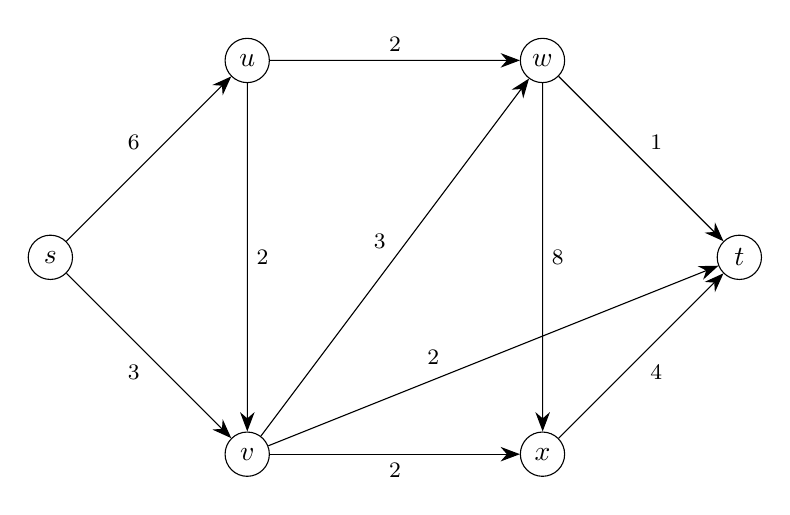
\begin{tikzpicture}[scale=2.5]
		\node[vertex] (s) at (1,1) {$s$};
		\node[vertex] (u) at (2,2) {$u$};
		\node[vertex] (v) at (2,0) {$v$};
		\node[vertex] (w) at (3.5,2) {$w$};
		\node[vertex] (x) at (3.5,0) {$x$};
		\node[vertex] (t) at (4.5,1) {$t$};
	
		\draw[directed] (s) to [edge label =6] (u);
		\draw[directed] (s) to [edge label'=3] (v);
		\draw[directed] (u) to [edge label =2] (v);
		\draw[directed] (u) to [edge label =2] (w);
		\draw[directed] (v) to [edge label =2,pos=0.4] (t);
		\draw[directed] (v) to [edge label'=2] (x);
		\draw[directed] (v) to [edge label =3] (w);
		\draw[directed] (w) to [edge label =1] (t);
		\draw[directed] (w) to [edge label =8] (x);
		\draw[directed] (x) to [edge label'=4] (t);
	\end{tikzpicture}
\end{center}

\noindent Do the following.
\begin{enumerate}[label=(\alph*)]
    \subsection{Problem 11\ref{ff3a}}
    \item \label{ff3a} Consider the flow-augmenting path $s \to u \to v \to t$. Push as much flow through the flow-augmenting path and draw the updated flow network below (we have provided a tikzpicture in the LaTeX comments that you can use and just modify the labels on the edges, or you may hand-draw and embed an image).

\begin{proof}[Answer]
This would be the maximum amount of flow that can be pushed through on this flow-augmenting path. This is due to the fact that on the edges of $u \to v, v \to t$ the maximum amount of flow that can be pushed on these edges is 2.
%If you wish, you may un-comment the tikzpicture below (remove the \begin{comment} and \end{comment} lines) and modify
%the edge weights. You may also hand-draw and embed an image

%Include an Image: \includegraphics{ImageFileName}
%Include an Image and Rotate 90 degree: \includegraphics[angle=90]{ImageFileName}
%Include an Image, Rotate by 180 degrees, and scale by 50\% \includegraphics[scale=0.5, angle=90]{ImageFileName}


\begin{center}
	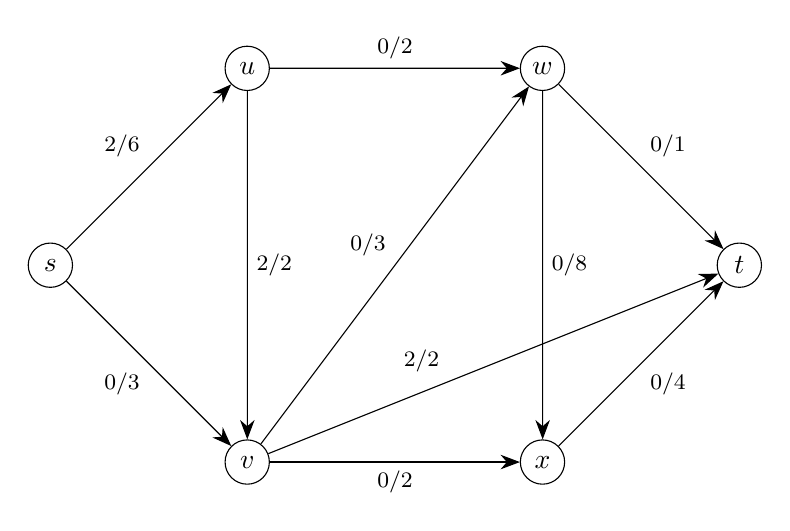
\begin{tikzpicture}[scale=2.5]
		\node[vertex] (s) at (1,1) {$s$};
		\node[vertex] (u) at (2,2) {$u$};
		\node[vertex] (v) at (2,0) {$v$};
		\node[vertex] (w) at (3.5,2) {$w$};
		\node[vertex] (x) at (3.5,0) {$x$};
		\node[vertex] (t) at (4.5,1) {$t$};
	
		\draw[directed] (s) to [edge label =2/6] (u);
		\draw[directed] (s) to [edge label'=0/3] (v);
		\draw[directed] (u) to [edge label =2/2] (v);
		\draw[directed] (u) to [edge label =0/2] (w);
		\draw[directed] (v) to [edge label =2/2,pos=0.4] (t);
		\draw[directed] (v) to [edge label'=0/2] (x);
		\draw[directed] (v) to [edge label =0/3] (w);
		\draw[directed] (w) to [edge label =0/1] (t);
		\draw[directed] (w) to [edge label =0/8] (x);
		\draw[directed] (x) to [edge label'=0/4] (t);
	\end{tikzpicture}
\end{center}
\end{proof}

\newpage
    \subsection{Problem 11\ref{ff3b}}
    \item \label{ff3b} Find a flow-augmenting path starting from the updated flow configuration from your answer to part (a). Then do the following: (i) clearly identify both the new flow-augmenting path and the maximum amount of flow that can be pushed through said path; and then (ii) push as much flow through the flow-augmenting path and draw the updated flow network below.

    \begin{proof}[Answer]
    The new flow-augmenting path would be from $s \to u \to w \to t$. This path would have a maximum amount of flow of 1. It would have a maximum amount of flow of one because on the edge from $w \to t$ the capacity is only 1, so thus it restricts the rest of our path to only allow us to push a maximum flow of 1 through this path.
%If you wish, you may un-comment the tikzpicture below (remove the \begin{comment} and \end{comment} lines) and modify
%the edge weights. You may also hand-draw and embed an image

%Include an Image: \includegraphics{ImageFileName}
%Include an Image and Rotate 90 degree: \includegraphics[angle=90]{ImageFileName}
%Include an Image, Rotate by 180 degrees, and scale by 50\% \includegraphics[scale=0.5, angle=90]{ImageFileName}


\begin{center}
	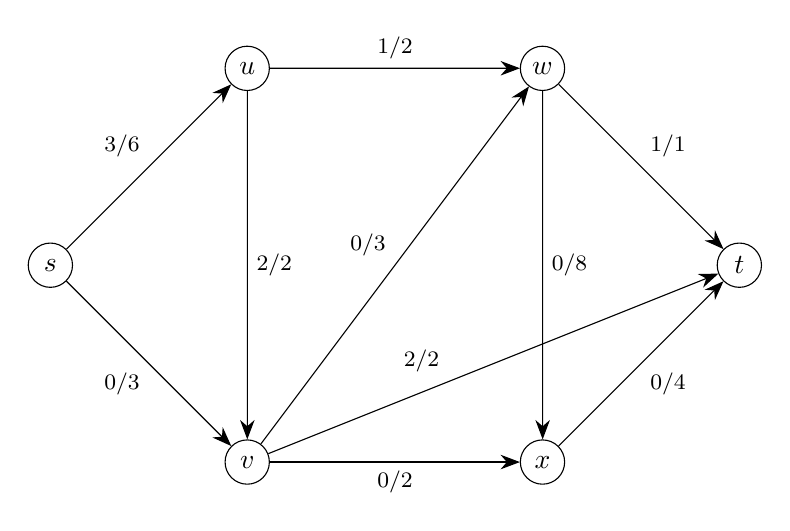
\begin{tikzpicture}[scale=2.5]
		\node[vertex] (s) at (1,1) {$s$};
		\node[vertex] (u) at (2,2) {$u$};
		\node[vertex] (v) at (2,0) {$v$};
		\node[vertex] (w) at (3.5,2) {$w$};
		\node[vertex] (x) at (3.5,0) {$x$};
		\node[vertex] (t) at (4.5,1) {$t$};
	
		\draw[directed] (s) to [edge label =3/6] (u);
		\draw[directed] (s) to [edge label'=0/3] (v);
		\draw[directed] (u) to [edge label =2/2] (v);
		\draw[directed] (u) to [edge label =1/2] (w);
		\draw[directed] (v) to [edge label =2/2,pos=0.4] (t);
		\draw[directed] (v) to [edge label'=0/2] (x);
		\draw[directed] (v) to [edge label =0/3] (w);
		\draw[directed] (w) to [edge label =1/1] (t);
		\draw[directed] (w) to [edge label =0/8] (x);
		\draw[directed] (x) to [edge label'=0/4] (t);
	\end{tikzpicture}
\end{center}

\end{proof}




\newpage

    \subsection{Problem 11\ref{ff3c}}
    \item \label{ff3c} Find a flow-augmenting path starting from the updated flow configuration from your answer to part (b). Then do the following: (i) clearly identify both the new flow-augmenting path and the maximum amount of flow that can be pushed through said path; and then (ii) push as much flow through the flow-augmenting path and draw the updated flow network below.

    \begin{proof}[Answer]
    The new flow-augmenting path would be $s \to v \to w \to x \to t$, with a maximum amount of flow being 3. The maximum amount of flow is only 3 because from the edges of $s \to v, v \to w$ the capacity for these edges are only 3, thus we can only push a maximum flow of 3 through this path. 
%If you wish, you may un-comment the tikzpicture below (remove the \begin{comment} and \end{comment} lines) and modify
%the edge weights. You may also hand-draw and embed an image

%Include an Image: \includegraphics{ImageFileName}
%Include an Image and Rotate 90 degree: \includegraphics[angle=90]{ImageFileName}
%Include an Image, Rotate by 180 degrees, and scale by 50\% \includegraphics[scale=0.5, angle=90]{ImageFileName}


\begin{center}
	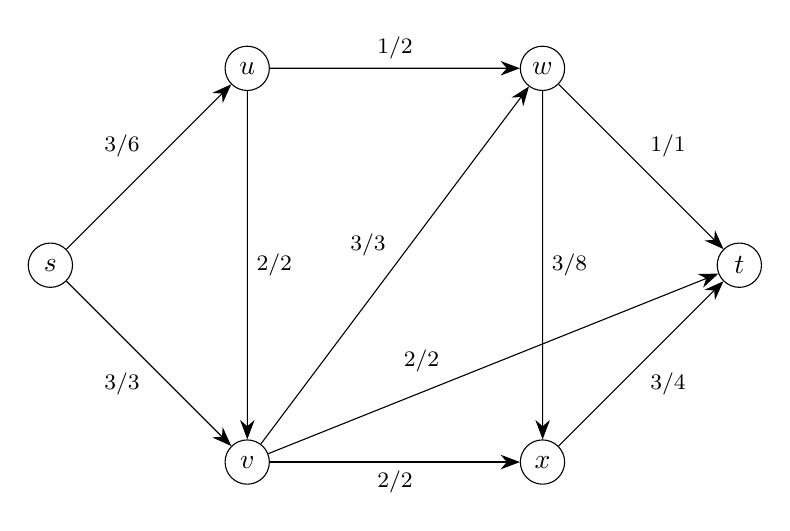
\begin{tikzpicture}[scale=2.5]
		\node[vertex] (s) at (1,1) {$s$};
		\node[vertex] (u) at (2,2) {$u$};
		\node[vertex] (v) at (2,0) {$v$};
		\node[vertex] (w) at (3.5,2) {$w$};
		\node[vertex] (x) at (3.5,0) {$x$};
		\node[vertex] (t) at (4.5,1) {$t$};
	
		\draw[directed] (s) to [edge label =3/6] (u);
		\draw[directed] (s) to [edge label'=3/3] (v);
		\draw[directed] (u) to [edge label =2/2] (v);
		\draw[directed] (u) to [edge label =1/2] (w);
		\draw[directed] (v) to [edge label =2/2,pos=0.4] (t);
		\draw[directed] (v) to [edge label'=2/2] (x);
		\draw[directed] (v) to [edge label =3/3] (w);
		\draw[directed] (w) to [edge label =1/1] (t);
		\draw[directed] (w) to [edge label =3/8] (x);
		\draw[directed] (x) to [edge label'=3/4] (t);
	\end{tikzpicture}
\end{center}
\end{proof}




\newpage


\newpage
    \subsection{Problem 11\ref{ff3d}}
    \item \label{ff3d} Using the flow configuration from part (c), finish executing the Ford--Fulkerson algorithm. Include the following here: (i) your flow network, reflecting the maximum-valued flow configuration you found, and (ii) the corresponding minimum capacity cut. There may be multiple minimum capacity cuts, but you should identify the one corresponding to your maximum-valued flow configuration. Then (iii) finally, compare the value of your flow to the capacity of the cut. \\

    \begin{proof}[Answer]
    Our final flow-augmenting path would be from  $s \to u \to w \to x \to t$, with a maximum capacity of 1. This path would only have a maximum capacity of 1 because from the edge $u \to w$ we have already pushed a flow on one through it thus, it can only hold a maximum flow of 1. 
    %%%%%%%%%%%%%%%%%%%%%%%%%%%%%%%%%%%%%%%%%%%%%%%%%%%%%%%%%%%%%%%%%%%%%%%%%%%%%%%
    % YOUR ANSWER GOES HERE: type your answer in below                             %
    %%%%%%%%%%%%%%%%%%%%%%%%%%%%%%%%%%%%%%%%%%%%%%%%%%%%%%%%%%%%%%%%%%%%%%%%%%%%%%%
    %If you wish, you may un-comment the tikzpicture below (remove the \begin{comment} and \end{comment} lines) and modify
%the edge weights. You may also hand-draw and embed an image

%Include an Image: \includegraphics{ImageFileName}
%Include an Image and Rotate 90 degree: \includegraphics[angle=90]{ImageFileName}
%Include an Image, Rotate by 180 degrees, and scale by 50\% \includegraphics[scale=0.5, angle=90]{ImageFileName}



\begin{center}
	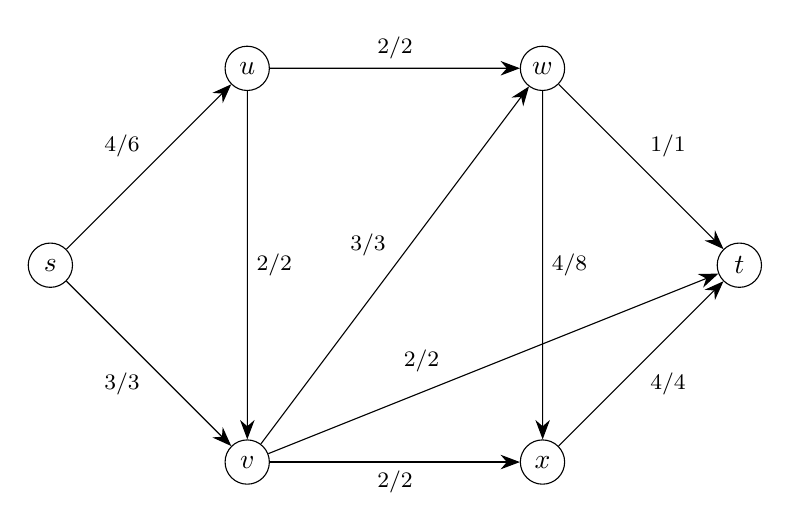
\begin{tikzpicture}[scale=2.5]
		\node[vertex] (s) at (1,1) {$s$};
		\node[vertex] (u) at (2,2) {$u$};
		\node[vertex] (v) at (2,0) {$v$};
		\node[vertex] (w) at (3.5,2) {$w$};
		\node[vertex] (x) at (3.5,0) {$x$};
		\node[vertex] (t) at (4.5,1) {$t$};
	
		\draw[directed] (s) to [edge label =4/6] (u);
		\draw[directed] (s) to [edge label'=3/3] (v);
		\draw[directed] (u) to [edge label =2/2] (v);
		\draw[directed] (u) to [edge label =2/2] (w);
		\draw[directed] (v) to [edge label =2/2,pos=0.4] (t);
		\draw[directed] (v) to [edge label'=2/2] (x);
		\draw[directed] (v) to [edge label =3/3] (w);
		\draw[directed] (w) to [edge label =1/1] (t);
		\draw[directed] (w) to [edge label =4/8] (x);
		\draw[directed] (x) to [edge label'=4/4] (t);
	\end{tikzpicture}
\end{center}
\end{proof}
    
\end{enumerate}

\end{required}



%%%%%%%%%%%%%%%%%%%%%%%%%%%%%%%%%%%%%%%%%%%%%%%%%%

\end{document} % NOTHING AFTER THIS LINE IS PART OF THE DOCUMENT


